\section{Introduction}
% Short abstract introduction here about this section (can be done when finished)

\subsection{Background}
\label{introduction-background}
% What is SeaDataCloud's exact problem? Make the problem clear so that our solution fits the problem. Try to look at it from all angles, like an os3 teacher would

Large data infrastructures such as SeaDataNet and CS3 are responsible for managing diverse data sets across the globe. These data sets are made available to a large number of users. In this section we will discuss these data infrastructures and the technical challenges they face at the moment.

SeaDataNet is a distributed marine data infrastructure network for managing the large and diverse data sets collected by the oceanographic fleets and the automatic observation systems. Reliable and fast marine data access is of importance for marine research and required for various studies, which varies from climate change research to off shore engineering. SeaDataNet started the SeaDataCloud project in 2016. Their aim is to advance and increase the usage of SeaDataNet's services by adopting cloud and high performance computing technology for better performance \cite{sdc}. SeaDataNet connects together more than a hundred data centres from eight European marine institutes in different geographical domains, aiming at preserving and making reusable marine observations ranging from ocean physics to chemistry and biology.

SeaDataCloud's current infrastructure is a centralized solution, as the current cache is a central catalogue which duplicates the entire data repository. Data consumers use host-to-host-connections (TCP/IP) to pull data from this cache, which could cause congestion with many concurrent data consumers. Data is pushed into SeaDataCloud's infrastructure by different data providers. Their current infrastructure is shown in figure \ref{fig:sdc_cur} and assigns a PID, which can be of any type, to each object that is pushed into the cache to uniquely identify an object. Data providers are not bound to a specific PID, thus different PID types are used. Each with their own naming schema.

CS3 is another case of a community that brings together users, researchers, developers, 
technology- and service providers of on-premise cloud services as well as large cloud service companies.
CS3 is dedicated to emerging cloud synchronization and sharing services 
to enable on-premise file sync/share services for researchers to share, transfer
and synchronize data in a simple but powerful way.

The CS3 community has been growing for the last three years and currently includes
around hundred institutions and companies from around the world.
One of the most important topics and technical challenge of CS3 services is interoperability. 
Development of interoperability protocols is important to provide data 
sharing capabilities for all users across all institutions in the field of education and research.

As mentioned, these data infrastructures cope with technical challenges at the moment. One of the technical challenges is the distribution of the data across the communities. The issue is that the data is distributed by different data providers across these communities, each with their own
naming schema. Therefore, interoperability across different naming schemas has to be achieved. Users should be able to request data across these communities, without having to cope with different schemas for data they request. Another technical challenge is to serve this data 
to a large number of users. The current approach can potentially cause congestion and delays with
many users consuming data from the highlighted distributed data infrastructures. On top of that, the large number of users is still growing. In section \ref{tech-oview} we highlight state of the art technologies to deal with these challenges. We will create a design which achieves interoperability across different naming schemas and alleviates network latency and congestion.

\begin{figure}[H]
\centering
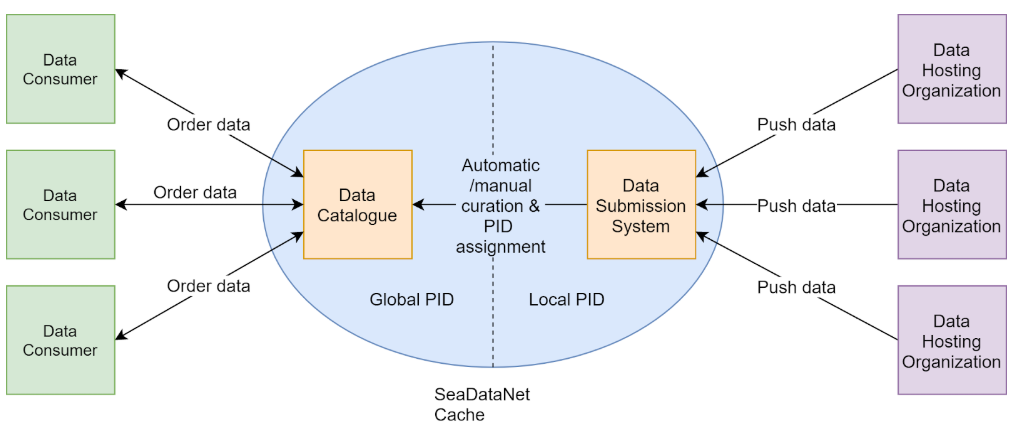
\includegraphics[scale=0.6]{Images/SDC_current.png}
\caption{SeaDataCloud's current infrastructure.}
\label{fig:sdc_cur}
\end{figure}

\subsection{Related technologies}
In this section we will briefly analyze and explain related technologies based on the problem statement from section \ref{introduction-background}. We will compare key properties of these technologies and based on the analysis and the process of elimination we will define the relevant technologies for this research.

\subsubsection{What is a PID?}\label{pid-intr}
Shortly after the introduction of the WWW, Tim Berners Lee (its creator) proposed to the IETF to use the URI as the naming schema for identifying contents on the web. This proposal got rejected by the IETF, due to the fact that it does not allow users of the web to change the URI of the web contents when moving the web contents to another location. This lead to the use of URLs as the naming schema to identify web content. 
%In this paper, the term Web content refers to a digital object.
 
The use of URLs was no issue at the early stages of the web, but several studies have found out that approximately 50\% of the URLs in scholarly publications fail to retrieve the digital object after a period of seven to ten years, where users of the web began to experience the problem of a broken link, or the so called "link rot" problem \cite{rot-link1, rot-link2}. This is a situation where a user fails to retrieve the web content by its URL, due to the fact that the location of the web content has been changed \cite{icn-bd, ark-id}. 

Therefore, the first PID systems emerged in the mid-1990s shortly after the introduction of the web itself. A PID is a long-lasting, permanent reference to digital objects. Traditional identifiers, such as the bibliographic identifier ISBN will not be interpreted as a hyperlink by web browsers. For example the string \texttt{ISBN 951-45-9942-X} has to be expressed as a HTTP URI in the form of \texttt{http://urn.fi/URN:ISBN:951-45-9942-X} to be a persistent link to the resource. As shown in the persistent link, the term URN is used, which is an example of a PID type that is used for object identification. In section \ref{pid-types} we will describe PID types in more detail. When using a PID, a user who requests the digital resource can trust that the correct digital resource is retrieved, even if the location where it resides has been changed \cite{pid-oview}.

\subsubsection{Data distribution technologies}
\label{introduction-ndn}
When the internet was conceived it was designed for host-to-host communication. This means that in order to retrieve data, a host needs to retrieve the data from an IP. Nowadays the internet is increasingly data-oriented rather than host-oriented. For example, in 2018 15\% of the worldwide average bandwidth use was consumed by Netflix, with regional peaks often reaching 40\% \cite{introduction-netflix}. With many users requesting the same video (or content in general), congestion can occur, degrading the user experience. Data locality sits on top of that problem, since data needs to cross distance as well, resulting in latency. Several technologies and methods have been developed to assist in efficient data distribution to improve performance. A few notable examples are CDNs, ICNs and BitTorrent.

CDNs have become a popular solution to decrease network latency \cite{lee2012towards}. In essence a CDN places content closer to its users. This is done by caching data in multiple geographical locations which are reachable over IP (often via anycast). These caches provide faster delivery of e.g. HTML pages, JavaScript files, style sheets, images, and videos. The key benefits of this solution are improved web content load times and increasing the availability and redundancy. Furthermore, CDNs can serve as a mitigation for DDoS attacks \cite{cloudflare-cdn}.

ICNs are another solution for data distribution \cite{jacobson2009networking}. However, ICNs employ a different networking methodology. An overlay is created on top of e.g. IP. In this overlay, data is identified and forwarded based on a globally unique hierarchical name rather than an IP (location). This removes the need to retrieve data from a specific IP address, which provides mobility as well. The data distribution is made possible by the use of caching. Intermediary ICN nodes may cache data objects along the network path. The ICN communication model is consumer-driven, meaning that the consumer initiates queries and thus the in-network caching. ICN nodes can be of any class such as mobile phones, laptops or dedicated ICN nodes with specific hardware for increased performance. This means that once data is retrieved from the original publisher and cached in a local network, it can be shared with neighboring peers. Furthermore, due to cryptographic signatures, the data can be verified in the network and/or application layer. Thus, providing provenance authentication of the data, even if the data came from a third party. Since data is retrieved by name and not location, traditional DDoS attacks are mitigated as well.

BitTorrent shares similarities with ICN \cite{mastorakis2017ntorrent}. Data can be downloaded from neighboring peers and the content can be verified with cryptographic hashes. However, BitTorrent tries to determine the best peers based on trail-and-error. The protocol 'chokes' and 'unchokes' peers in order to guess the best quality peers to download from. This method is applied because BitTorrent has no knowledge of the network topology and routing policies. Furthermore, data can only be verified in the application layer. This means that corrupted data is only identified and discarded when it reached the consumer. 

Based on the problem statement from section \ref{introduction-background} and the analyses of these related technologies; ICN offers the best solution. This is due to that ICN provides easier distribution of data by being able to forward data by name rather than IP and makes use of in-network caching. Thus, when a climate scientist downloads a large dataset from his or her's workstation, that data may then be cached locally. Other scientists interested in the data can then take advantage of this local cache. Thus, the original data publisher won't have to send the same data twice, lowering the chance of congestion. Furthermore, ICN has the ability to detect corrupt data in the network layer by the use of cryptographic hashes. Therefore, corrupt data isn't forwarded once corruption is detected and thus saving bandwidth. ICN is the common architectural idea which has spawned several different implementations. Based on the related work (section \ref{introduction-related-work}) we decided to use NDN, which is discussed in more detail in section \ref{overview-ndn}.

\subsection{Related work}
\label{introduction-related-work}
% Related work summary, only stuff that's directly relevant for our research. Other references can be made later by simply mentioning them. Avoid summarizing related work in too much detail, keep it clear and concise. We need to show our contribution, not what others did.
% short intro about this section needed, connecting the pid and ndn part


In this section we will provide an overview of existing solutions for PID interoperability and known NDN performance and scalability issues and solutions.

\subsubsection{PID interoperability}
\label{introduction-pid}
In 2014, Karakannas researched the efficiency of ICN for delivering big data with PIDs \cite{icn-bd}. PIDs are used in big data infrastructures to identify digital content and research data. The research proposed a mapping architecture for resolving PIDs to ICN names. Karakannas proposed to use a PID to NDN mapping server for every PID type instead of implementing the translation on the clients browser. For the latter, the researcher states that translation of a PID to NDN name will be highly depended on the clients NDN browser, which needs to be updated every time a new PID schema would be introduced \cite{icn-bd}.
%The research results showed that in-network caching can offer significant performance benefits, when the cache size of the network elements that perform in-network caching is bigger than the Big Data object size. 

In 2017, Mousa researched the fetching and sharing of DOI objects with ICN such as NDN. 
The researcher's approach focused only on DOI identified objects within NDN networks, which was possible. Mousa states that there are many other different PID systems that can also be identified and translated for compatibility with the NDN naming schema. Furthermore, the researcher explains that difference in NDN naming of different PID providers must be taken into account, such that the correct prefix is used within NDN to identify specific PID types. For example, using the prefix \texttt{"doi/"} within NDN for DOI identified objects.
In the researcher's design, the translation happens in the consumers browsers. The consumer has the choice to either request the digital object by its NDN name or PID \cite{ndn-app-aware}.

Zhao et al. progressed the research done by Karakannas \cite{icn-bd} and Mousa \cite{ndn-app-aware} and proposed an architecture to map PIDs into the naming schema of NDN. Their proposed solution is called NDN-as-a-service for PID data objects (NaaS4PID) and supports one PID type. This solution is composed out of three key components \cite{icn-resteam}:
\begin{itemize}
  \item PID2NDN gateway; primarily responsible for resolving PIDs to NDN names.
  \item NDN4PID router image; an NDN node that implements a virtualized NDN router.
  \item NDN4PID manager; automates the management of the NDN overlay in\newline cloud or e-infrastructure.
\end{itemize}

Olschanowsky et. al. researched translating climate modeling schema filenames, used by CMMAP applications at Colorado State University, to an NDN compatible 
naming schema. The researchers designed an NDN name translator to support the data management needs of CMMAP. The NDN name translator incorporates a naming schema that is designed to be compatible with existing climate modeling schemas, like CMIP5. While allowing for some flexibility for project-specific requirements. They explain that NDN names for climate data should be both expressive and human readable. The advantages of long expressive names versus short easy to remember names have to be balanced.
The researchers state that every data provider should publish a data prefix which acts as a globally
routable prefix within NDN covering all of the data made available by the provider. This complies with Mousa, who stated that NDN naming of different PID providers must be taken into account. The researchers consulted with CMMAP climate scientists and confirmed that these naming rules are acceptable for their datasets and are appropriate for global distribution. 
However, the translation is not as easy as taking the filename only and translating it into an NDN name. To construct appropriate NDN names to uniquely identify data of a specific model, the filename to NDN translator needs information gleaned from the filesystem path, filename and metadata mined from the data itself. This information is processed by a filename to NDN name mapping schema to be used for CMMAP filenames. Therefore, some intelligence is expected in their translators.
Figure \ref{fig:cmmap_ndnn} shows the translation of a CMMAP to an NDN name. In this example it is shown that after the prefix, which identifies the provider \url{"/coupled/control/CMMAP/"}, the NDN translated name contains additional information next to the input filename \cite{ndn-clim}.
%, which is parsed from metadata or information that resides in the data itself \cite{ndn-clim}. 
They further state that since NDN naming is flexible and virtually any appropriate
translation schema can be plugged into, it is possible to support many naming schemas as long as the 
name can be broken down in hierarchical components.

\begin{figure}[H]
\centering
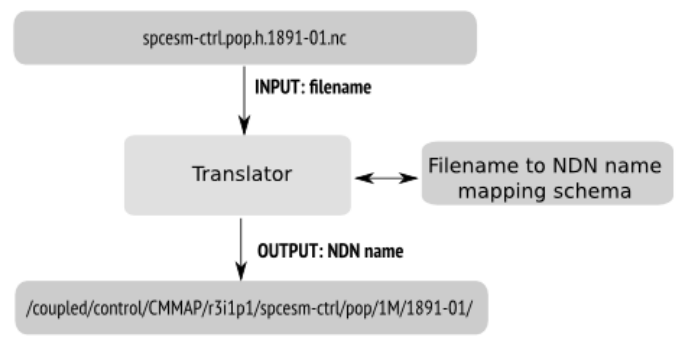
\includegraphics[scale=0.4]{Images/cmip2ndn.png}
\caption{CMMAP to NDN name translator.}
\label{fig:cmmap_ndnn}
\end{figure}

The research done by Fan et. al. utilizes a catalog which holds the the translation of NDN names. Users query the catalogue to receive an NDN name. This process is fairly lightweight since the catalog's only concern is to add or remove names rather than dataset synchronization. The researchers use datasets of the CMIP5 climate modeling schema for their research and encourage to use the climate modeling schema as a prefix for an NDN name. 
Their catalog design can support the needs of any community, which can be seen as a data provider described earlier. The catalog is able to define and use consistent naming schemas.
The researchers concluded that their catalog facilitates NDN name discovery and that data management can be made easier for scientific communities as long as they converge on common naming schemas \cite{ndn-man}. 

\subsubsection{NDN performance and scalability}
\label{introduction-related-work-ndn}
ICN is the common architectural idea of forwarding packets based on their name rather than destination (IP) \cite{jacobson2009networking}. Research done by Karakannas \cite{icn-bd} concluded that NDN was the only ICN approach that published a specification and workable software to experiment with. As of writing this report, we concluded that this conclusion is still valid. Therefore, this research used NDN for experimentation.

James McCabe's "Network Analysis, Architecture, and Design" \cite{mccabe2010network} book offers a systems methodology approach towards network design. The approach is described in McCabe as "seeing the network part of a larger system, with interactions and dependencies between the network and its users, applications and devices". The methodology put forward by McCabe is to design a network based on several inputs and outputs:
\begin{itemize}
    \item Analysis: What do users/services require? How are the relationships composed between these components?
    \item Architecture: Which technology and topology choices support the users/services needs? Based on this, create high-level, end-to-end structure of the network.
    \item Design: Determine the physical detail of the architecture based on output of the previous steps.
\end{itemize}

The inputs and outputs used in this method are intended to be iterative and by no means define a final architecture design. This is due to the fact that requirements, technology and user behaviour can change and with that the network design. Section \ref{overview-mccabe} provides a more detailed overview of this method and section \ref{planning-ndn} describes how it's applied for this research.

NDN is relatively new and thus not much is known yet about the performance in different scenarios. In order to plan a network, it would be necessary to know what works and doesn't work for NDN. Large NDN testbeds are still rare. However, there is sufficient research available that focused on particular design choices of NDN. Research done by Lim et al. \cite{lim2018ndn} at a large existing testbed located in the USA \cite{ndn-testbed-status} highlighted a few lessons learned. Lim et al. setup the first intercontinental NDN testbed with the intent to see the benefits for big science (big data). They implemented a name translator for climate-science data, which translated CMIP files to an NDN compatible name. They concluded that NDN provided performance improvements compared to classical climate data delivery techniques based on TCP/IP. A network was used for testing which provided direct links across the USA. The research concluded that NDN over UDP does not properly support large NDN packets (\textgreater 64kB). According to the research this was due to UDP's properties of not applying congestion control and proper packet retransmission and resulted in unsatisfying performance. The loss of a single UDP segment resulted in the retransmission of a large NDN data packet, consisting out of many UDP packets. However, NDN over TCP demonstrated a more reliable and faster performance due to the allowance of larger dynamic window sizes and congestion control. Native NDN congestion control is still an open research area \cite{ren2016congestion}, as of writing this report, no proposal has been implemented.

The performance benefits of NDN concluded by Lim et al. correlates with research done by Shannigrahi et al. at the USA-based large hadron collider network \cite{shannigrahi2015named}. Shannigrahi et al. achieved a 71\% reduction in the average delay per data chunk compared to a no-caching case. Shannigrahi et al. conducted NDN caching simulations \cite{shannigrahi2017request}. They concluded that a small cache of several gigabytes already reduces the network load. However, as expected, increasing the cache towards 1TB reduced the network load even further. However, this reduction of load wasn't proportional to the cache size. They concluded in their research that a 1GB NDN cache at the edge of the NDN network can already significantly improve data distribution and reducing the network load from servers. The average file size in use was 1.3GB.

Furthermore, in NDN several caching, cache replacement and forwarding strategies can be used to fine-tune performance. Koulouzis et al. researched these strategies and concluded that the 'leave copy everywhere' caching strategy provided the best performance ratio between cache size to data object size for generic data usage. However, 'leave copy down' and 'leaving copies with probability' performed best for delivering big data objects. Koulouzis et al. also concluded that the ascending ordering of data objects enhances network performance when combined with the 'least recently used' caching strategy. This was concluded based on observations that if large objects were requested first, the cache replacement algorithm would make room by overwriting files already in the cache, resulting in cache misses. When small files were requested first, more cache hits were measured. As for cache size, the researchers recommended a cache size at least twice the size of the biggest data object in the network. Yuan et al. \cite{yuan2012scalable} researched the performance of NDN forwarding. They used the CCNx application\footnote{\url{https://wiki.fd.io/view/Cicn}} to perform experiments. Their research concluded that packets with long names degraded performance. After profiling the software they measured that the NDN name decode operation took 35.46\% of the entire program running time. So et al. \cite{so2013named} developed a method to achieve fixed lookup times with variable length names. In order to achieve this goal they explored the application of hash tables to do name lookup. Furthermore, they explored the possibility to do this in hardware by using a Cisco ASR9000 router with the integrated service module. This module ran 64-bit Linux, using 2 Intel 2.0GHz hexa-core Westmere EP (Xeon) processors with hyper-threading. Additionally it included up to three 2TB SSD drives. With their experiments they managed to forward 20Gbps of real NDN traffic. Tortelli et al. \cite{tortelli2013performance} researched the effectiveness of two opposite forward strategies; flooding and best-route (with and without caching). Several experiments let them to the conclusion that there are pros and cons in each forwarding strategy. But that it's difficult to determine the most performant forward strategy.

\subsection{Research question}
\label{introduction-research-question}
% Based on the use case and related work, what is it that we will research and why? What is it that we want to answer?
With the technical challenges in mind as described in section \ref{introduction-background} and the related work from section \ref{introduction-related-work}, we will answer the following research questions. 

\begin{itemize}
	\item How to make the PID and NDN namespace interoperable?
\end{itemize}

We will research different PID types to find a feasible solution to implement NDN interoperability with future PID types. Based on the problem statement of section \ref{introduction-background}, 
we will explore interoperability methods.

%This is in response to the highlighted data infrastructures described in section \ref{introduction-background}, which cope with interoperability across different data providers. This is due to the fact that the different data providers use different naming schema to serve objects to data consumers.

%Next to this, SeaDataCloud's planned solution needs to support multiple PID types, as PIDs that get assigned to objects in their infrastructure can be of any type, we will look into supporting different PID types to find a feasible solution to implement future PID types easily. This will be answered with the following sub-questions.
\begin{itemize}
    \item[--] How to support different PID types?
    \item[--] How to incorporate extensibility for future PID schemas?
\end{itemize}


SeaDataCloud's current infrastructure is a centralized host-to-host solution which could cause a lot of congestion with many concurrent users. And CS3's community is growing with more data consumers. Therefore, our planned solution incorporates NDN to overcome the issues of traditional host-to-host oriented techniques. Therefore, we will research the planning of an NDN network with scalability in mind. To achieve this, the following research question needs to be answered.   
\begin{itemize}
    \item How to plan and manage an NDN network's life cycle with scalability in mind?
\end{itemize}

To answer this research question we need to analyze the known scalability problems in NDN. Furthermore, the term scalability needs to apply to manageability as well. If scaling up or down in terms of resources is made uncomplicated, the efforts needed to manage this infrastructure needs to stay the same.
\begin{itemize}
    \item[--] Which NDN scaling problems are known?
    \item[--] Which method can be used to plan an NDN network?
    \item[--] How to deploy an NDN network with scalability in mind?
\end{itemize}

\subsection{Scope}
\label{introduction-scope}
% What will we do and what will we skip? Based on what's already done in related work and our research question

Based on related work (section \ref{introduction-related-work}) and the research question (section \ref{introduction-research-question}) we defined the following scope for our research. We will develop a method to make the PID types URN, Handle and DOI interoperable with the NDN namespace. This will be done to demonstrate that interoperability of different PID types is possible within NDN. The reason we do not cover more PID types in our methodology is because with the aforementioned PID types we can already prove that PID interoperability is possible. We also aim to define a solution where future PID types can be added uncomplicated. Therefore, the interoperability goals are to demonstrate that different PID types can be used within NDN. 

The planning of the NDN network has the following goals. Based on the known performance limitations (section \ref{introduction-related-work-ndn}) and the data infrastructures discussed in section \ref{introduction-background}, we will develop a method for planning and deployment. This includes a proof of concept where, based on NDN's adaptability, the network can be adjust for scale in both performance but also in terms of manageability. The proof of concept will be limited to existing software solutions.

\subsection{Report structure}
To-do after finishing our paper.

%After having introduced the reader to the concepts and related work of our researched subjects, this paper starts with a technical overview of the technology being used in section \ref{tech-oview}. In this section we will describe PIDs, NDN, McCabem, TOSCA and virtualization in more depth and more detail.
%The paper continues by describing our methodology in section \ref{method}, which includes showing our proposed model which describes how interoperability is achieved. Furthermore, this section will bring the attention of how to plan a NDN network by using orchestration tools such as McCabe and TOSA and how NDN scalability is achieved. 
%After the aforementioned section we will get to the results in section \ref{res} to show the results we got from the experiments based on our methodology.
%The discussion then follows in section \ref{disc} to discuss difficulties we came across during our research and what advice can be given to the reader.
%Finally we enforce the value of this research by concluding our findings in section \ref{conc} and wrap up our research by giving insight in future work for the readers in section \ref{fut} to think about and perhaps getting picked up by other researchers. 

% To guide the reader into what's to come, can be done only when whole report is done